\section{為什麼特首和特區政府總是民望低落?}

無論是行政長官的選舉方式或管治團隊的組成過程,均對行政長官在一般市民心目中建立認授和管治威信十分不利。當行政長官的認授基礎薄弱,市民就不會主動支持,於是即使施政有道也不會受到讚賞,施政失誤的話卻會成為眾矢之的。因此,行政長官和特區政府的民望自然下跌易,回升難。

到目前為止,香港特區尚未出現過一位卸任時民望比就任的時候高的行政長官,民望低落似乎是成為行政長官必然要面對的咀咒。香港大學民意調查計劃自前港督彭定康就任開始便一直調查香港市民對香港政府領導人的評分。彭定康上任是的評分是52.5,最高點為64.1,卸任時為59.7,仍比上任時要高。進入特區年代,每一位行政長官的評分在卸任時都比上任時要低。董建華就任的時候有64.5分,到了二零零三年中期曾跌得低至36.2,而到了他辭職下台時也只回復到47.9。曾蔭權上任的時候評分高達72.3,但之後一直下跌,到卸任時更低至39.2。繼任的梁振英在上任時的評分已是各人中最低的52.5,到他卸任時則是比曾蔭權最低點還要低的38.1。如果只是一位行政長官面對評分滑落,還可以說只是他個人不濟。但經過二十年的實踐,行政長官的民望不停下跌已成為常態,這現象就得從制度上找尋答案。

\begin{figure}[htbp]
    \centering
    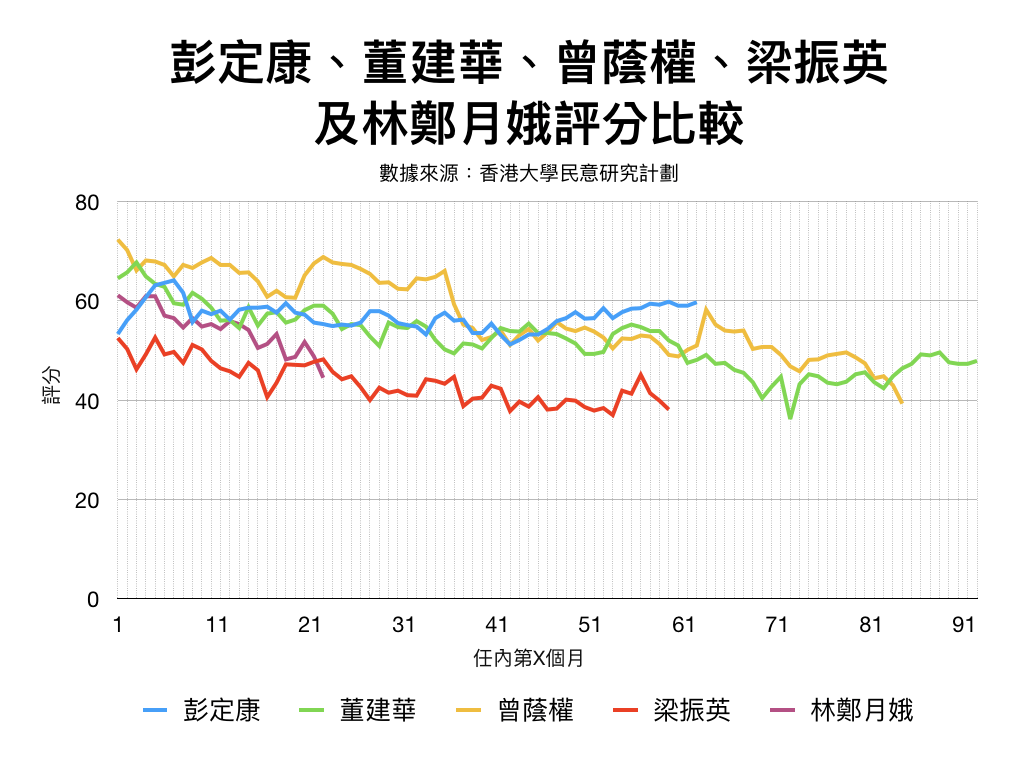
\includegraphics[width=0.7\textwidth]{c19/h-klesson1-028.png}
    \caption{自董建華以來每屆特首的評分都是從上任以來一直下降} 
\end{figure}

上文提到選舉制度上的控制使行政長官無法如民主社會中從選舉中取得認授,而這問題在管治團隊的組成過程被進一步深化。表面上行政長官擁有很多權力,但這些權力往往都需要其他人的支持才能實行。當這些人選出現問題,行政長官本身也會受到質疑。而經過十多年的實踐,學界發現管治團隊難以得到市民支持,原因並不限於個別官員本身的問題,而是整個制度有鼓勵劣幣驅逐良幣的傾向,政府無法匯聚人才。當官員表現令人咋舌,政府民望每況愈下就是意料中事。

先說行政與立法關係。《基本法》明確規定行政長官受立法會的監督,具體來說包括制定、修改或廢除法律,審核和通過財政預算和公共開支,監察政府施政和質詢主要官員等,必要時更有權彈劾行政長官。由於行政長官不是由香港市民選出的,立法會議員對他再嚴厲也不用擔心得罪曾經投他一票的人。相反,立法會議員自己必須每隔四年接受選舉洗禮,當政府本身的認授低落時,他們沒有任何誘因站在政府的一邊,反而充滿誘因落井下石,好讓得到選民的支持。換言之,香港的政治制度本身十分鼓勵立法會議員對特首嚴厲,相對於責怪這些議員為求套取選票而去攻擊政府,應反問為何制度沒有提供調節的誘因。

當然,在一個正常的民主制度之下,總統或行政首長在立法機關當中總會一定數量的支持者。例如當美國總統是民主黨黨員,則他大約可確定國會內的民主黨黨籍議員大多數都會支持他的施政。當他的提議交到國會審議時,可假定會有一定數量來自民主黨的支持,然後再去爭取中間游離的議員的支持,而不用從零開始爭取國會過半數的贊成票。不過在香港,要成為行政長官,卻要符合一條相當奇怪的規定:《行政長官選舉條例》第三十一條要求行政長官當選人必須聲明不是任何政黨的成員。這個安排原則上是要行政長官超越黨爭,實際上卻使得政府在立法會一票也沒有的,每一位議員都是潛在的反對派。畢竟就算行政長官本身沒有政黨背景,但立法會議員,特別是直選產生的議員,很多都有黨派背景。政府無論想做任何事情,都得在立法會尋求各個黨派的支持。

自特區成立以來,各任行政長官都很快意識到這個制度問題,於是便產生了「執政聯盟」的概念。簡單來說,就是雖然行政長官自己沒有政黨背景,但立法會中有個別黨派和他的關係比較好,行政長官可以借用這些黨派的議員在立法會內為政府護航。因此,這些黨派往往會被稱為建制陣營甚至是「保皇黨」。但這個做法相對於行政長官正式從屬於一個政黨有明顯的分別:「執政聯盟」往往十分鬆散,未必時時能提供穩定支持。如果行政長官本來就從某個政黨出身的,他和他的政黨先有理念上的互相認同,過去黨務工作和選戰中也曾互相支持,自然能建立出可靠和穩定的互信關係。香港的「執政聯盟」卻不是這樣的。行政長官和「執政聯盟」的政黨之間不一定有共同理念,過去甚至可以在政治上並不友好。政黨本身長期存在,行政長官每位最多做十年,所以「執政聯盟」某程度上有得罪行政長官的本錢,反正總有一天人走茶涼。過去就曾多次發生「執政聯盟」叛變的事件,在最後關頭拒絕支持政府的提議,政府發現未能在立法會夠票通過之下只好臨時撤回建議,表現極為難堪。

\begin{figure}[htbp]
    \centering
    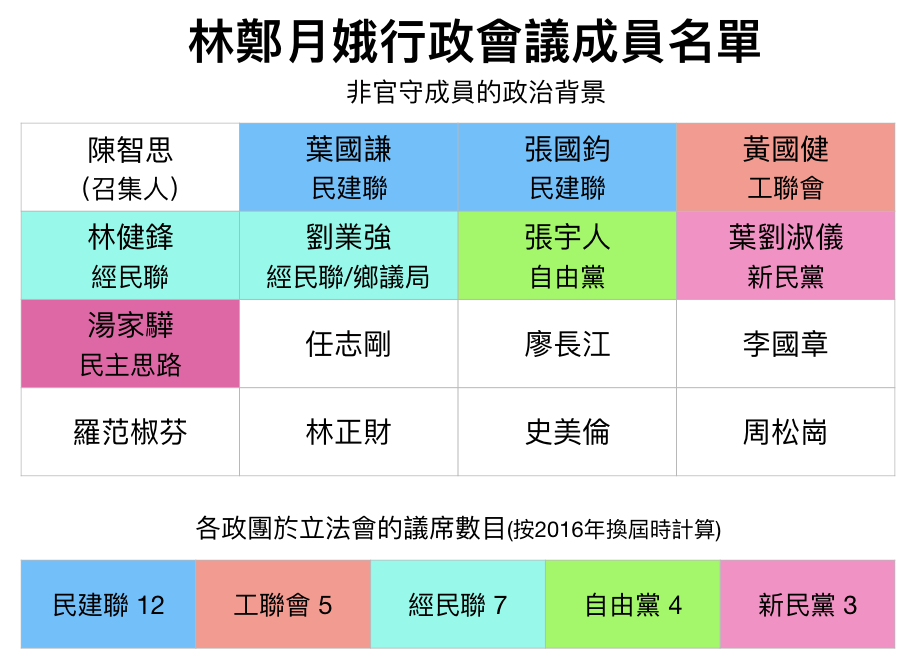
\includegraphics[width=0.7\textwidth]{c19/h-klesson1-030.png}
    \caption{林鄭月娥的行政會議變成拉攏建制陣營政黨的工具} 
\end{figure}

「執政聯盟」的問題歸根究底,在於這些政治結盟並不是建立在政治理念之上,而是一場利益交易。政黨參與之後,能優先知道政府接下來的施政重點,於是他們便可反過來演一場戲,預早向政府「爭取」相關政策。當這些政策得到落實之後,政黨便可向選民吹噓自己的政績。反過來,當政府爆出巨大醜聞,而且嚴重到有可能影響他們的選舉部署時,他們又會抽身而出,重拾監督政府的角色。在這個關係當中,無論是行政長官或是「執政聯盟」的政黨都希望得到最大的好處,大家都不會真心誠意地希望「榮辱與共」。在市民眼中,他們也很明白「執政聯盟」的政黨為政府護航,本身不一定是出於真心信服相關政策,而只是政治立場的表現,說服力也就大打折扣。

「執政聯盟」不單影響行政立法關係,更會影響人事任命,進一步打擊行政長官和政府的公信力。

政府政策必須要得到立法會的通過,而不少民選議員都是靠罵政府來贏取議席,所以政府無法不依靠「執政聯盟」的支持。然而這些「執政聯盟」也不笨,他們很明白政府如果沒有他們的支持就寸步難行,對政府的要求自然會越來越多。一開始的時候,「執政聯盟」往往只體現在個別政黨的領袖人物成為行政會議的成員,理由是方便行政長官可以在政策尚未出台之前便能先參考這些政黨的意見,好讓日後推出的時候能得到他們的支持。不過,近年來「執政聯盟」更常體現在政府官職的政治任命當中,給予公眾用人為親的印象。

在討論人事任命問題前,得先解釋香港特區政府的官制。在特區政府剛成立的時候,為了保持管治穩定,整個政府只換了一個人,由英國政府派來的港督彭定康,變成由中國政府委命的董建華。至於董建華轄下的所有官員,則全數來自公務員的華人文官系統。在香港,公務員是指政府長期僱傭關係下的僱員。以特區首任政務司司長陳方安生為例,她在一九六二年大學畢業加入政府當政務官,在不同部門工作,輾轉晉升為彭定康之下的第一人,然後過渡為董建華之下的第一人。

問題是正正因為陳方安生連同所有高級官員都是由公務員系統中層層升遷上來,董建華基本上沒有任何空間選擇由誰為他做事。當行政長官連點將的權力也沒有,面對負責官員陽奉陰違的時候就難以換人。此外,為了確保公務員行事不偏不倚,任用條款規定除非犯下離天大錯,否則必可續任,要懲處的話最多也只能將之投閒置散。如是者,即使公眾認為個別官員失職,行政長官也不能將之立即革走。例如在一九九八年新機場開幕後一片混亂,輿論普遍認為要有高級官員負責,卻沒有一人因此而下台。及後在二零零零年又發生公屋短樁醜聞,面對立法會的不信任動議,不屬公務員制度的房屋委員會主席王䓪鳴黯然下台,公務員體系內的時任房屋署署長苗學禮卻拒絕跟隨,施政失誤時政治責任由誰承擔的問題變得十分明顯。與此同時,經過特區首五年的運作後,董建華發現自己儘管是特區的行政長官,卻可以被整個政府的行政官僚架空,於是便想到改革政府高層的管治架構,並於二零零二年實施「主要官員問責制」。

特區政府的架構本身就傾向美式的總統制,行政權和議會分開產生,問責制的出現可謂讓香港的政府架構進一步向美式政治靠攏。在美國,每次換總統也要同時重新任命約四千人,因為總統需要他信任和與他合拍的副手,而這些副手也需要他們信任和與他們合拍的助理。問責制的出現,讓行政長官可以如美國總統一樣自己選擇主要官員的人選。在一開始的時候,問責制只包括三名司長和十一名政策局長,現時已擴張至每名司局長可再有數名副手,如副局長和政治助理。

問責制的其中一個原意是要製造「旋轉門」,高級官員不一定要在公務員隊伍尋找,也可以讓社會中有名望而又和行政長官理念相通的人才加入政府,和他共同進退,也就是所謂的「政治委任」。當有新政策要推動的時候,這些問責高官就負責政治推銷和協商的工作,而公務員則回復其中立的執行角色。如果這些問責高官的工作出了什麼問題,行政長官也可以中途換人以向公眾交代。

表面上問責制是個有效的安排,但放在香港的制度框架卻帶來了很多問題。美國的政治委任制度有兩個特點和香港不一樣。首先,美國的總統有政黨支持,香港沒有;第二,美國的高級政治委任官員都要由民選的參議院確認,香港的問責高官不需要立法會確認,反而需要中央政府任命。這兩個差別決定了當同一個制度來到香港時,效果有明顯落差。

由於美國的政黨長期存在而且輪流執政,能成為聚集人才的地方。例如當民主黨的候選人當選總統,就可以在民主黨的黨員及其友好之間尋找高級官員,而這些人和總統之間的理念都會想近,而且較有互信。到了總統任滿或落台的一天,這些前高級官員不會一下子樹倒猢猻散,因為他們知道下次選舉說不定又會選出一個民主黨黨員,他們會再有機會大展拳腳。香港的行政長官由於沒有政黨支持,要找高級官員也不知道可以從什麼地方找。有能力擔任此等職位的社會賢達,理念和行政長官不一定配合,雙方也沒有互信。更重要的,和上面「執政聯盟」的討論一樣,他們很明白行政長官的任期有限,自己的任期不會比行政長官長,甚至如果中途有什麼意外的話更要下台。面前眾多不確定因素,這些社會賢達一般都不願意放棄已有的高薪厚職和政治清譽。

此外,由於問責官員的任命權在中央政府,行政長官只有提名權,實行起來便會出現中央政府否決行政長官提名人選的問題。這種情況不會得到官方確認,因為每次特首在提出正式提名之前必定會先和中央政府溝通,免除人選不獲委任的尷尬。不過每屆新的行政長官上任時,新聞中常會流傳個別人選被中央政府否決的說法,打擊新任行政長官和問責官員的威信。

問責制實行十多年來,問責高官可說是越來越難找,願意出任者的社會地位和能力於是也變得越來越低,反過來拖累政府形象。新當選行政長官的林鄭月娥在競選時就曾經說過要帶來管治新風格,又以自己有較多的社會賢達支持來攻擊對手。可是到了她當選之後,卻公開表示擔心找不到一個完整的問責高官團隊和她一起就任,結果願意就任者絕大多數都是從上屆政府過檔,談不上有什麼「新朝新氣象」。

\begin{figure}[htbp]
    \centering
    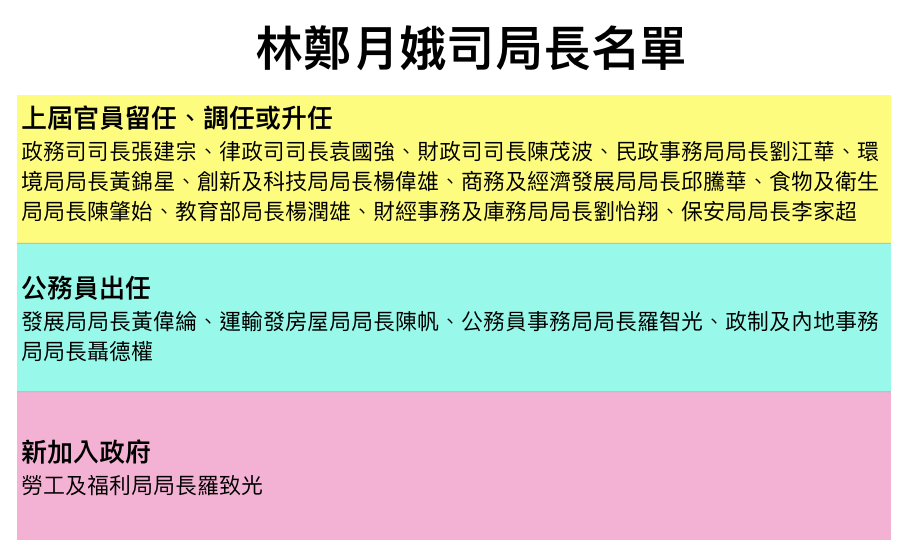
\includegraphics[width=0.7\textwidth]{c19/h-klesson1-031.png}
    \caption{林斯月娥幾乎找不到新人加入管治團隊} 
\end{figure}

當願意做問責官員的人越來越少,任命權的問題便顯得更為致命。社會對問責制的期望是市民能向政府問責,然而由於任命權在中央政府而不在立法會,民意其實無從有效地向問責高官問責。當行政長官提名一些明顯沒有相關能力的人選成為問責高官,又或一些問責高官做出明題違反市民期望的事情時,民意無從阻擋。以曾任發展局局長的陳茂波為例,他上任時被揭發曾在舊區經營劏房,以及在發展區囤積農地,與他的職位有品格甚至利益上的衝突。雖然他就任以來在民意調查當中的反對度一直遠高於支持度,而他的個人問題更導致市民質疑政府的城市發展計劃,但是他不止無需辭去官職,後來更晉升為財政司司長。

說到這兒,問題又回到「執政聯盟」的利益交易質疑了。由於問責高官的任命完全取決於行政長官和中央政府,在沒有制衡之下很容易便和行政會議成員一樣成為政治交易的籌碼,用作鞏固權力之用。當行政長官要尋求政黨在立法會提供穩定支持,除了提供行政會議成員的席位外也要安排個別的政治任命官職,使問責制被批為變相政治酬庸。以教育局首任政治助理楊哲安為例,本身並非來自教育專業,沒有相關的學術成就,當時也未曾當選過民意代表,和政治的最大關聯是他的父親楊孝華曾任自由黨的立法會議員,而自由黨當時為政府拉攏合作的對象。

說到這兒,不難發現香港的政治制度有一個很明顯的先天缺陷:在香港,從政本身不能成為一項志業,而對其他專業人才來說走進政壇則是一件高風險低回報的事情。制度上的不足使得香港政府從行政長官到政治助理都做不到唯才是用,政治忠誠更為重要。所以,有能力的人大多不願意去碰這淌混水,寧願明哲保身。當管治團隊表現拙劣,各種醜聞無日無之,則政府的支持度自然難有翻身之日。

\rule[-10pt]{15cm}{0.05em}

伸延閱讀:

Fong B (2014) Ten Years of Political Appointments in Hong Kong — The Challenges and Prospects of Developing a Political Appointment System under a Semi-Democratic Regime, 2002-2012, Cheng JYS (ed) \textit{New Trends of Political Participation in Hong Kong}. City University of Hong Kong Press.